\documentclass[article,11pt]{abntex2}
\usepackage[utf8]{inputenc}
\usepackage{graphicx}
\usepackage[T1]{fontenc}
\usepackage[brazil]{babel}
\usepackage{lipsum}
\usepackage{multicol}
\usepackage{helvet}
\usepackage{microtype}
\usepackage{subcaption}
\usepackage{amsmath}
\usepackage[american,siunitx]{circuitikz}
\usetikzlibrary{calc,shapes,chains}
\usepackage[a4paper,headsep=0pt,headheight=25mm,margin=25mm]{geometry}
\usepackage[absolute]{textpos}
\usepackage{fancyhdr}
\usepackage{fancyvrb}
\renewcommand{\headrule}{}

\renewcommand{\section}[1]{\par\bigskip\noindent\MakeUppercase{\textbf{#1}}\par}


\addto\captionsbrazil{
    \renewcommand{\figurename}{FIGURA}
	\renewcommand{\tablename}{TABELA}
	\renewcommand{\bibname}{}
	\renewcommand{\bibsection}{}
}
\renewcommand{\sc}{\scshape}
\renewcommand{\bf}{\bfseries}
\lhead{\hspace*{-17mm}
\includegraphics[width=38.56mm]{Conict.png}}
\chead{\parbox[b][6ex][t]{10cm}{\centering\textsf{\textbf{4º Congresso Pós-Graduação do IFSP - 2019}}}}
\rhead{\parbox[b][12ex][c]{35mm}{
\includegraphics[width=35mm,height=12.12mm]{IFSP.jpg}}\hspace*{-15mm}}
\fancyfoot{}
\SingleSpacing

\begin{document}
	\thispagestyle{fancy}
	\begin{center}{\bfseries TÍTULO (Times New Roman, 11, Negrito, Centralizado)}\end{center}
	
	\begin{textblock}{4.6}[1,0](16.4,1.15)
	\fbox{\begin{minipage}{45mm}\centering\footnotesize\color{red}Não informe o nome dos\\autores na etapa de avaliação. Apenas na versão final.\\\vspace{1.5ex}
	O resumo expandido deve ter\\\textbf{no máximo cinco páginas}\\\vspace{1.5ex}
	\tiny{Remova este quadro antes do envio}\end{minipage}}
	\end{textblock}
	
	\begin{center}FULANO C. SILVA$^1$, AUTOR$^2$, AUTOR$^3$, AUTOR$^4$\\
	(Times New Roman, 11, Centralizado, Máximo quatro autores)\end{center}
	{\footnotesize $^1$ Graduando em Tecnologia de Análise e Desenvolvimento de Sistemas, Bolsista PIBIFSP, IFSP, Câmpus Cubatão, fulanocsilva@ifsp.edu.br. (Times New Roman, 9, Justificado)\\
	$^2$ \\
	$^3$ \\
	$^4$ \\
	Área de conhecimento (Tabela CNPq): 1.03.03.04-9 Sistemas de Informação}
	\begin{center}
		Apresentado no\\
		4º Congresso de Pós-Graduação do IFSP\\
		27 e 28 de novembro de 2019 - Sorocaba-SP, Brasil
	\end{center}
	\noindent\textbf{RESUMO:} O propósito destas instruções é orientar aos autor(es) quanto à formatação dos resumos expandidos a serem submetidos ao Congresso de Inovação, Ciência e Tecnologia do Instituto Federal de Educação, Ciência e Tecnologia de São Paulo. Os documentos devem ser redigidos de acordo com as normas para elaboração do resumo expandido. O arquivo de submissão deverá estar desbloqueado no formato \emph{portable document format} (pdf) compatível com o Adobe Acrobat Reader™. O texto deve iniciar na mesma linha do item, ser claro, sucinto e, obrigatoriamente, explicar o(s) objetivo(s) pretendido(s), procurando justificar sua importância (sem incluir referências bibliográficas), os principais procedimentos adotados, os resultados mais expressivos e conclusões, contendo no máximo 200 palavras. Não deverá conter fórmulas e citações e referências bibliográficas. O resumo expandido apresentado no evento será publicado nos Anais (\textit{ISSN}: 2178-9959). O texto com as instruções e em parênteses devem ser removidos do documento final. (Times New Roman, 11, Justificado, Máximo 200 palavras).\par
	\bigskip\noindent\textbf{PALAVRAS-CHAVE:} máximo de seis, separadas por ponto e vírgula (;), procurando não repetir palavras do título, escritas em letras minúsculas. (Times New Roman, 11, Justificado).\par
	
	\begin{center}{\bfseries TÍTULO EM INGLÊS (Times New Roman, 11, Negrito, Centralizado)}\end{center}
	\noindent\textbf{ABSTRACT:} Tradução do resumo para a língua inglesa. (Times New Roman, 11, Justificado).\par
	\bigskip\noindent\textbf{KEYWORDS:} Tradução das palavras-chave para a língua inglesa. (Times New Roman, 11, Justificado).\par
	
	\section{Introdução}
	No máximo 20 linhas, evitar divagações, utilizando bibliografia apropriada para formular os problemas abordados e a justificativa da importância do assunto, deixando claro a(s) hipótese(s) e o(s) objetivo(s) do trabalho. (Times New Roman, 11, Justificado, Máximo 20 linhas).\vspace{3cm}
	
	\section{Material e Métodos}
	Os materiais e métodos utilizados no desenvolvimento da pesquisa devem ser adequadamente descritos. (Times New Roman, 11, Justificado).\par
	
	\textbf{Modelo de equação:}
	\begin{equation}
	    I_C=\frac{F\cdot9,81}{A}\cdot10^{-6}
	\end{equation}
	em que,
	\begin{itemize}[itemsep=-5pt]
	    \item[$I_C$] - índice de cone, MPa;
	    \item[$F$] - força, kgf;
	    \item[$A$] - área do cone, m2.
	\end{itemize}

	\section{Resultados e Discussão}
Ilustrações e gráficos devem ser apresentados com tamanho e detalhes suficientes para a composição gráfica final, preferivelmente na mesma posição do texto. \par
\textbf{Gráficos:} devem apresentar-se sem bordas, descritos com o mesmo tipo e tamanho de letras contidas no texto e a legenda na posição inferior do mesmo. A numeração deve ser sucessiva em algarismos arábicos.\par
\textbf{Tabelas:} evitar tabelas extensas e dados supérfluos; adequar seus tamanhos ao espaço útil do papel e colocar, na medida do possível, apenas linhas contínuas horizontais; suas legendas devem ser concisas e autoexplicativas. Na discussão, confrontar os dados obtidos com a literatura. (Times New Roman, 11, Justificado).\par
\textbf{Modelo de Figuras:}
	\begin{figure}[h]
		\centering
		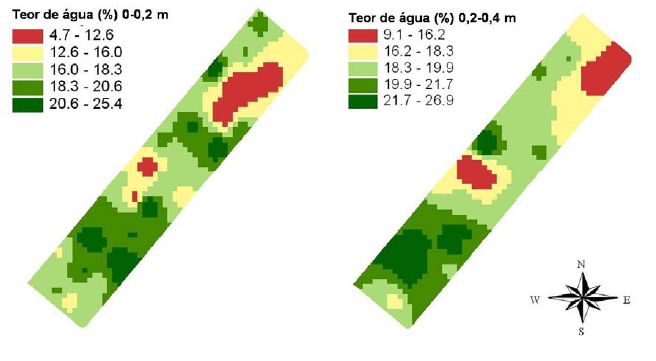
\includegraphics[width=.6\textwidth]{Fig1.png}
		\caption{Mapas de teor de água das camadas de 0-0,2 e 0,2-0,4 m de profundidade.}\label{fig:Fig1}
	\end{figure}
	\begin{figure}[h]
		\centering
		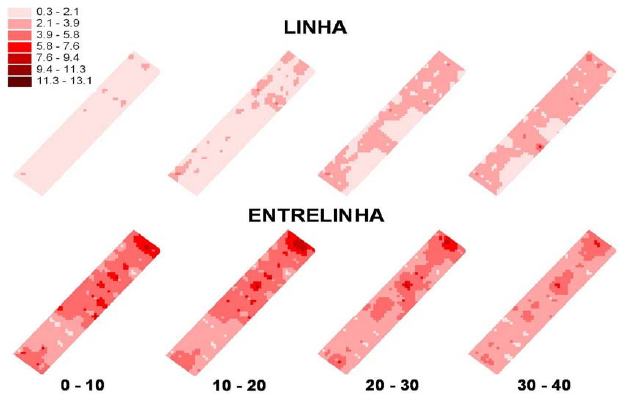
\includegraphics[width=.6\textwidth]{Fig2.png}
		\caption{Mapas do índice de cone (MPa) referente aos dados coletados nas diferentes profundidades nas linhas e nas entrelinhas da cultura da cana.}\label{fig:Fig2}
	\end{figure}\clearpage
	
\textbf{Modelo de Tabelas:}
	\begin{table}[h]
	    \centering
	    \caption{Análise do $I_C$ nas linhas (L) e entrelinhas (E) de cana nas diferentes profundidades amostradas pelo índice de cone.}\label{tab:Tab1}
	    \begin{tabular}{*{9}{c}}\hline
	       Profundidades (m)  & \multicolumn{2}{c}{0 a 0,1} & \multicolumn{2}{c}{0,1 a 0,2} & \multicolumn{2}{c}{0,2 a 0,3} & \multicolumn{2}{c}{0,3 a 0,4} \\\hline
	         & L & E & L & E & L & E & L & E\\
	       Média (MPa) & 1,39$^{**}$ & 4,28$^{**}$ & 1,86$^{**}$ & 4,29$^{**}$ & 2,20$^{**}$ & 3,83$^{**}$ & 2,46$^{**}$ & 3,44$^{**}$ \\
	       CV (\%) & 54 & 57 & 55 & 54 & 46 & 49 & 48 & 43 \\\hline
	    \end{tabular}
	    \legend{$^{**}$: valores significativos para o nível de significância de 1\% pelo teste de Tukey; L – linhas; E – entrelinhas.}
	\end{table}
	
    \begin{table}[h]
        \centering
        \caption{Correlações entre índice de cone ($I_C$) e teor de água ($U_D$) nas camadas de 0-20 e 20-40 cm nas linhas e nas entrelinhas da cultura da cana.}\label{tab:Tab2}
        \begin{tabular}{c c c}\hline
             & $I_C$ x $U_D$ (0-20 cm) & $I_C$ x $U_D$ (20-40 cm)\\\hline
           Linhas  & -0,1256 \textsuperscript{n.s.} & -0,2426  \textsuperscript{n.s.} \\
           Entrelinhas  & -0,4317  \textsuperscript{n.s.} & -0,4882  \textsuperscript{n.s.} \\\hline
        \end{tabular}
        \legend{\textsuperscript{n.s.}:valores não significativos para o nível de significância de 5 e 1\%.}
    \end{table}
	
	\section{Conclusões}
	Devem basear-se exclusivamente nos resultados do trabalho. Evitar a repetição dos resultados em listagem subsequente, buscando, sim, confrontar o que se obteve com os objetivos inicialmente estabelecidos. (Times New Roman, 11, Justificado).
	
	\section{Agradecimentos}
	Inserir após as conclusões, de maneira sucinta. Se o projeto for financiado por alguma agência de fomento, citar a fonte. (Times New Roman, 11, Justificado).

	
	\section{Referências}
	As referências devem ser listadas em ordem alfabética. Veja os seguintes exemplos:
	\nocite{*}
	\bibliographystyle{acm}
	\bibliography{references.bib}
	
\end{document}